\documentclass[10pt,a4paper]{article}
\usepackage[margin=2.2cm]{geometry}
\usepackage{amsmath,amssymb,bm}
\usepackage{graphicx}
\usepackage{booktabs}
\usepackage{tabularx}
\usepackage{tikz}
\usetikzlibrary{arrows.meta,calc}
\usepackage[numbers,sort&compress]{natbib}
\usepackage{microtype}
\usepackage[hidelinks]{hyperref}
\usepackage{cleveref}

% units without siunitx
\newcommand{\un}[1]{\,\mathrm{#1}}
\newcommand{\vect}[1]{\bm{#1}}
\newcommand{\hatn}{\vect{n}}
\newcommand{\tagCAD}{\textsc{cad}}
\newcommand{\tagDS}{\textsc{ds}}
\newcommand{\tagAS}{\textsc{as}}
\newcommand{\tagDR}{\textsc{dr}}

\title{Physics and Modelling of the Ball Balancing Platform Simulator\\[2pt]
\large Model specification, derivations and verification}
\author{Ball Balancing Platform project}
\date{Model version 1.0 --- \today}

\begin{document}
\maketitle

\begin{abstract}
This document specifies, completely and independently of its implementation, the physical
model behind the Ball Balancing Platform (BBP) simulator: the kinematics and dynamics of the
three-legged (3-RRS) parallel mechanism that tilts the plate, the hobby-servo actuators, the
rolling, slipping, sticking and bouncing of the ball on the moving plate (including its
rolling inertia), and the formation of the image seen by the camera that looks up through the
transparent plate. Every equation that the simulator integrates is stated here, every
parameter is listed with its source, and every simplification is named. The model is verified
against classical closed-form results---the $\frac{5}{7}g\sin\beta$ law of rolling, the
$\frac{2}{7}\Omega$ orbit of a ball on a turntable, the $\frac{5}{7}v_0$ transition from sliding
to rolling, Snell refraction through a slab---and the agreement is reported to machine
precision where the theory is exact.
\end{abstract}

\tableofcontents

%======================================================================
\section{Purpose and scope}
%======================================================================
The BBP is a teaching platform for computer vision and control. Students write a ball tracker
and a controller; the same code runs on the physical platform (on a DFRobot FireBeetle~2
ESP32-S3) and in a simulator they can use at home. For the simulator to be a fair stand-in for
the hardware, students must be able to see \emph{what} it assumes, even though the code that
implements it is not distributed. This document is that statement: the physics is transparent,
the implementation is not.

The simulated system comprises
\begin{enumerate}
  \item the \textbf{mechanism}: a level-able plate carried by three crank--rod legs
        (\cref{sec:geometry,sec:kinematics,sec:dynamics});
  \item the \textbf{actuators}: three position-controlled hobby servos driven by PWM
        (\cref{sec:servo});
  \item the \textbf{ball}: a rigid sphere in frictional, unilateral contact with the moving
        plate (\cref{sec:ball});
  \item the \textbf{camera}: an image sensor below the plate, seeing the ball through it
        (\cref{sec:camera}).
\end{enumerate}
\Cref{sec:numerics} describes how the equations are integrated, \cref{sec:verification} the
verification, and \cref{sec:limitations} what is \emph{not} modelled. The modelling of the
student-facing artificial delays and of processor execution time belongs to the software
framework and is specified separately.

\paragraph{Conventions.} Vectors are bold and, unless stated otherwise, expressed in the world
frame. SI units are used throughout; lengths in tables are given in millimetres where that is
clearer. A dot denotes a time derivative in the world frame. $[\vect a]_\times$ is the
cross-product matrix, $[\vect a]_\times\vect b=\vect a\times\vect b$. For a unit normal
$\hatn$, the tangential part of a vector is $\vect x_t=\vect x-(\vect x\cdot\hatn)\hatn$.
Parameter provenance is tagged \tagCAD{} (measured from the CAD model), \tagDS{} (component
datasheet), \tagDR{} (derived) and \tagAS{} (assumed; to be identified on the real platform).

%======================================================================
\section{Geometry from the CAD model}\label{sec:geometry}
%======================================================================
All geometric parameters are extracted automatically from the STEP assembly
\texttt{CAD/FullASSY.step} by a script (\texttt{tools/cad/extract\_geometry.py}) that
identifies the joints by their characteristic surfaces: the crank hub cylinders give the servo
axes, the crank-pin holes the lower joints of the rods, and the \(8\un{mm}\) balls the
spherical joints under the plate. The values are listed in \cref{tab:geometry}.

\begin{table}[h]
\centering
\caption{Geometry of the mechanism (\tagCAD). The world frame is the CAD frame: $z$ up, origin
on the central axis at the height of the plate's lower face in the as-modelled pose.}
\label{tab:geometry}
\begin{tabular}{llr}
\toprule
Quantity & Symbol & Value \\
\midrule
Leg azimuths & $\beta_i$ & $-150^\circ,\,-30^\circ,\,90^\circ$ \\
Radius of servo (crank) axes & $r_A$ & $44.007\un{mm}$ \\
Height of servo axes & $z_A$ & $-90.934\un{mm}$ \\
Crank length (axis to pin) & $L_1$ & $50.000\un{mm}$ \\
Rod length (pin to sphere centre) & $L_2$ & $118.598\un{mm}$ \\
Radius of spherical-joint circle & $r_B$ & $94.000\un{mm}$ \\
Depth of joint centres below plate top & $h_s$ & $13.598\un{mm}$ \\
Plate radius, thickness & $R_p,\ t_p$ & $100\un{mm},\ 5\un{mm}$ \\
Ball radius & $a$ & $10.000\un{mm}$ \\
Camera optical centre & $\vect C$ & $(0,0,-92.404)\un{mm}$ \\
Crank angle in the CAD pose & $\theta_{\mathrm{CAD}}$ & $-45.004^\circ$ \\
\bottomrule
\end{tabular}
\end{table}

\paragraph{Idealisation.} In the CAD assembly the mid-section is rotated by $0.47^\circ$, so
each leg plane passes $0.77\un{mm}$ beside the central axis. The model uses the design intent:
exact $120^\circ$ symmetry with leg planes through the axis. The forward kinematics of the
idealised model reproduces the CAD plate height in the CAD pose to within $2.6\un{\mu m}$
(\cref{sec:verification}), which bounds the effect of this idealisation.

\paragraph{Operating pose.} The CAD shows the cranks $45^\circ$ below horizontal. The simulator's
neutral pose has the cranks horizontal ($\theta_i=0$, servo pulse $1500\un{\mu s}$), where each
rod is vertical and perpendicular to its crank---the best force transmission. The plate top is
then at $h_0=41.263\un{mm}$, $133.67\un{mm}$ above the camera. Both choices are parameters.

\begin{figure}[h]
\centering
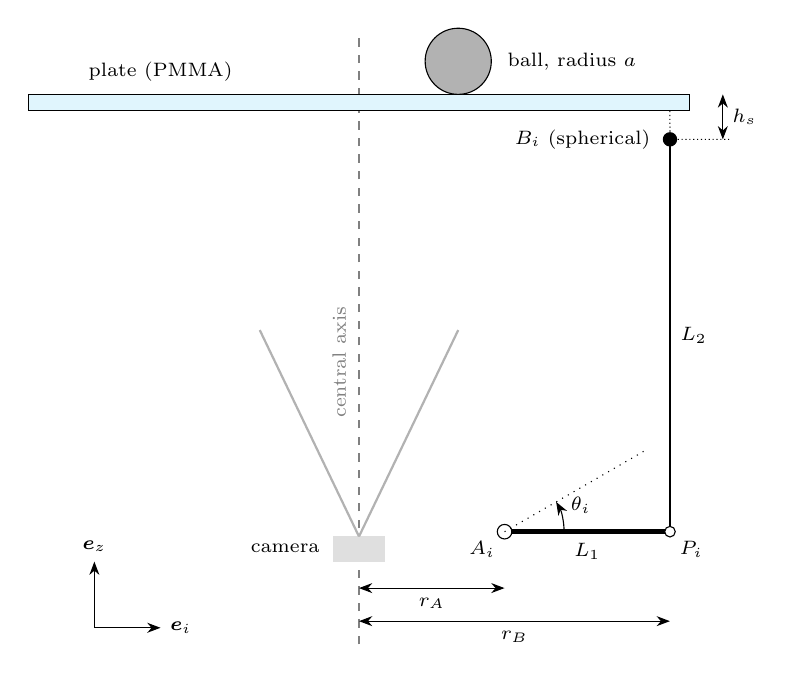
\begin{tikzpicture}[scale=0.042,>=Stealth]
  % central axis
  \draw[dashed,gray] (0,-125) -- (0,60);
  \node[gray,font=\scriptsize,rotate=90,anchor=south east] at (-1,-20) {central axis};
  % base level / pivot
  \fill[gray!25] (-8,-100) rectangle (8,-92.4);
  \node[left,font=\scriptsize] at (-9,-96) {camera};
  \draw[gray!60,thick] (0,-92.4) -- (-30,-30) (0,-92.4) -- (30,-30);
  % pivot A, crank, pin P
  \coordinate (A) at (44,-90.93);
  \coordinate (P) at (94,-90.93);
  \coordinate (B) at (94,27.66);
  \draw[line width=1.6pt] (A) -- node[below,font=\scriptsize]{$L_1$} (P);
  \draw[line width=1pt] (P) -- node[right,font=\scriptsize]{$L_2$} (B);
  \filldraw[fill=white] (A) circle (2.2);
  \filldraw[fill=white] (P) circle (1.6);
  \filldraw[fill=black] (B) circle (2.0);
  \node[below left,font=\scriptsize] at (A) {$A_i$};
  \node[below right,font=\scriptsize] at (P) {$P_i$};
  \node[left,font=\scriptsize] at (91,27.66) {$B_i$ (spherical)};
  % crank angle
  \draw[->] ($(A)+(18,0)$) arc (0:30:18);
  \node[font=\scriptsize] at ($(A)+(23,8)$) {$\theta_i$};
  \draw[dotted] (A) -- ($(A)+(50*0.866,50*0.5)$);
  % plate
  \fill[cyan!12] (-100,36.26) rectangle (100,41.26);
  \draw (-100,36.26) rectangle (100,41.26);
  \draw[densely dotted] (B) -- (94,36.26);
  \node[font=\scriptsize] at (-60,48) {plate (PMMA)};
  % ball
  \filldraw[fill=gray!60] (30,51.26) circle (10);
  \node[font=\scriptsize,right] at (42,51.26) {ball, radius $a$};
  % dimensions
  \draw[densely dotted] (B) -- (112,27.66);
  \draw[<->] (110,27.66) -- node[right,font=\scriptsize]{$h_s$} (110,41.26);
  \draw[<->] (0,-108) -- node[below,font=\scriptsize]{$r_A$} (44,-108);
  \draw[<->] (0,-118) -- node[below,font=\scriptsize]{$r_B$} (94,-118);
  % axes
  \draw[->] (-80,-120) -- (-60,-120) node[right,font=\scriptsize]{$\vect e_i$};
  \draw[->] (-80,-120) -- (-80,-100) node[above,font=\scriptsize]{$\vect e_z$};
\end{tikzpicture}
\caption{One leg in its vertical plane, drawn to scale in the neutral pose ($\theta_i=0$).
The servo turns the crank $A_iP_i$ about an axis along $\vect t_i$; the rod $P_iB_i$ is hinged
at $P_i$ about a parallel axis and ends in a spherical joint $B_i$ fixed to the plate. The
camera looks up through the transparent plate.}
\label{fig:leg}
\end{figure}

%======================================================================
\section{Kinematics of the 3-RRS mechanism}\label{sec:kinematics}
%======================================================================
Each leg is an actuated revolute joint (servo), a passive revolute joint (crank pin) and a
spherical joint (under the plate): a 3-RRS parallel mechanism with three degrees of freedom,
kinematically equivalent to the classical 3-RPS manipulator of
\citet{lee1988kinematic} in that every spherical joint is confined to a fixed vertical
plane \citep{tsai1999robot,merlet2006parallel}.

\subsection{Frames and loop-closure constraints}
Leg $i$ lies in the vertical plane through the central axis at azimuth $\beta_i$, spanned by
$\vect e_i=(\cos\beta_i,\sin\beta_i,0)^T$ and $\vect e_z$; its normal is
$\vect t_i=\vect e_z\times\vect e_i$. The servo axis passes through
$\vect A_i=r_A\vect e_i+z_A\vect e_z$ along $\vect t_i$, and the crank pin is at
\begin{equation}
  \vect P_i(\theta_i)=\vect A_i+L_1\left(\cos\theta_i\,\vect e_i+\sin\theta_i\,\vect e_z\right),
\end{equation}
with $\theta_i$ measured from the outward horizontal, positive when the pin rises.

The plate frame $P$ has its origin $\vect p$ at the centre of the plate's \emph{top} face and its
$z$ axis along the plate normal $\hatn=\vect R\vect e_z$; $\vect R$ maps plate to world
coordinates. The spherical joints sit at plate coordinates
$\vect b_i=(r_B\cos\beta_i,\ r_B\sin\beta_i,\ -h_s)^T$, i.e.\ at
$\vect B_i=\vect p+\vect R\vect b_i$. The plate pose must satisfy six constraints,
\begin{align}
  g_{2i-1}&=\frac{\lVert\vect B_i-\vect P_i(\theta_i)\rVert^2-L_2^2}{2L_2}=0
  &&\text{(rod length)}, \label{eq:rod}\\
  g_{2i}&=\vect t_i\cdot\vect B_i=0 &&\text{(joint in the leg plane)}, \label{eq:plane}
\end{align}
for $i=1,2,3$. The scaling of \eqref{eq:rod} gives both rows units of length, which keeps the
Newton iteration below well conditioned.

\subsection{Orientation: tilt-and-torsion angles}
Following \citet{bonev2002advantages}, the plate orientation is written as
\begin{equation}
  \vect R=\vect R_z(\phi)\,\vect R_y(\vartheta)\,\vect R_z(\sigma-\phi),
\end{equation}
where $\vartheta$ is the \emph{tilt} (angle between plate normal and vertical), $\phi$ the
\emph{azimuth} of the tilt and $\sigma$ the \emph{torsion}. The plate normal depends only on
$(\phi,\vartheta)$: $\hatn=(\sin\vartheta\cos\phi,\ \sin\vartheta\sin\phi,\ \cos\vartheta)^T$.
For the student interface the tilt is specified by two \emph{surface slope angles}
$(s_x,s_y)$---the angles the plate surface makes with the horizontal along the world $x$ and
$y$ directions---through $\hatn\propto(-\tan s_x,-\tan s_y,1)^T$. Unlike a pair of Euler angles
this definition does not depend on a rotation order.

\subsection{Zero torsion and parasitic translation}
Let $\vect p_J=\vect p-h_s\hatn$ be the centre of the joint circle. Substituting
$\vect B_i=\vect p_J+r_B\vect R(\cos\beta_i,\sin\beta_i,0)^T$ with $\sigma=0$ into
\eqref{eq:plane} and writing $\psi_i=\beta_i-\phi$ gives, after elementary trigonometry,
\begin{equation}
  -\sin\beta_i\,p_{J,x}+\cos\beta_i\,p_{J,y}=-\tfrac{r_B}{2}(1-\cos\vartheta)\sin 2\psi_i .
\end{equation}
For legs spaced by $120^\circ$, $2\beta_i\equiv 3\beta_1-\beta_i \pmod{2\pi}$, so the right-hand
side becomes $-\frac{r_B}{2}(1-\cos\vartheta)\sin(\gamma-\beta_i)$ with $\gamma=3\beta_1-2\phi$:
a first harmonic in $\beta_i$, exactly like the left-hand side. All three equations are
therefore satisfied by
\begin{equation}
  \sigma=0,\qquad
  \begin{pmatrix}p_{J,x}\\ p_{J,y}\end{pmatrix}
  =-\frac{r_B}{2}\,(1-\cos\vartheta)\begin{pmatrix}\cos\gamma\\ \sin\gamma\end{pmatrix}.
  \label{eq:parasitic}
\end{equation}
This mechanism is thus a \emph{zero-torsion} mechanism in the sense of
\citet{bonev2002advantages}: it never yaws, and it translates sideways by
$\frac{r_B}{2}(1-\cos\vartheta)$---$0.71\un{mm}$ at $10^\circ$ of tilt---in a direction that turns
at twice the tilt azimuth. The same result is known for the 3-PRS and 3-RPS families
\citep{carretero2000kinematic}. Heave $p_z$ is free.

\subsection{Inverse kinematics}
Given the desired normal $\hatn$ and plate-top height $h$, the pose follows from
\eqref{eq:parasitic}: $\vect R$ from $(\phi,\vartheta)$ with $\sigma=0$, $p_x,p_y$ from
$\vect p=\vect p_J+h_s\hatn$, and $p_z=h$. (The implementation refines $(p_x,p_y,\sigma)$ with a
few Newton steps on \eqref{eq:plane}, which makes it exact for any leg layout and changes
nothing for the symmetric one.) Each crank angle then follows in closed form. With the joint
centre expressed in leg-plane coordinates relative to the servo axis,
$u_i=\vect e_i\cdot\vect B_i-r_A$ and $v_i=B_{i,z}-z_A$, the rod-length condition
$(u_i-L_1\cos\theta_i)^2+(v_i-L_1\sin\theta_i)^2=L_2^2$ is solved by
\begin{equation}
  \theta_i=\operatorname{atan2}(v_i,u_i)-\arccos\frac{K_i}{\rho_i},\qquad
  K_i=\frac{u_i^2+v_i^2+L_1^2-L_2^2}{2L_1},\quad \rho_i=\sqrt{u_i^2+v_i^2},
\end{equation}
taking the branch of the assembled mechanism (crank pin outside and below the line
$A_iB_i$). The pose is reachable if and only if $|K_i|\le\rho_i$ for all legs.

\subsection{Forward kinematics}
Given $\vect\theta$, the pose is found by Newton's method on the six constraints
\eqref{eq:rod}--\eqref{eq:plane}. The unknown is updated as a twist
$\delta\vect x=(\delta\vect p,\delta\vect\varphi)$: $\vect p\leftarrow\vect p+\delta\vect p$,
$\vect R\leftarrow\exp([\delta\vect\varphi]_\times)\vect R$ (Rodrigues' formula), followed by
re-orthonormalisation. Since $\delta\vect B_i=\delta\vect p+\delta\vect\varphi\times\vect R\vect b_i$,
the rows of the constraint Jacobian $\vect\Phi_x$ are
\begin{equation}
  \frac{\partial g_{2i-1}}{\partial\delta\vect x}=\left[\vect d_i^T,\ (\vect R\vect b_i\times\vect d_i)^T\right],\quad
  \frac{\partial g_{2i}}{\partial\delta\vect x}=\left[\vect t_i^T,\ (\vect R\vect b_i\times\vect t_i)^T\right],
  \quad \vect d_i=\frac{\vect B_i-\vect P_i}{L_2}.
\end{equation}
In the simulator the iteration is warm-started from the previous time step and converges in
one or two iterations.

\subsection{Velocity Jacobian and singularities}
Differentiating the constraints gives $\vect\Phi_x\vect\xi+\vect\Phi_\theta\dot{\vect\theta}=\vect 0$
for the plate twist $\vect\xi=(\vect v_p,\vect\omega_p)$, where $\vect v_p$ is the velocity of
$\vect p$ and $\vect\omega_p$ the angular velocity. $\vect\Phi_\theta$ has a single non-zero
entry per leg, $\partial g_{2i-1}/\partial\theta_i=-\vect d_i\cdot\vect P_i'(\theta_i)$. Hence
\begin{equation}
  \vect\xi=\vect J\dot{\vect\theta},\qquad \vect J=-\vect\Phi_x^{-1}\vect\Phi_\theta\in\mathbb R^{6\times3}.
\end{equation}
The mechanism is singular when $\vect\Phi_\theta$ loses rank (a crank aligned with its rod,
\emph{type~I}) or when $\vect\Phi_x$ does (\emph{type~II}, the plate gains a degree of
freedom), following \citet{gosselin1990singularity}. Neither occurs in the working range; the
simulator stops with an error if one is reached.

%======================================================================
\section{Mechanism dynamics}\label{sec:dynamics}
%======================================================================
\subsection{Inertial model}
\begin{itemize}
  \item \textbf{Plate}: mass, centre of mass and inertia tensor from the CAD solid scaled by the
        density of PMMA, $\rho=1190\un{kg/m^3}$ (\tagAS{} material): $m_p=0.188\un{kg}$,
        $I_{xx}=I_{yy}=4.73\times10^{-4}$, $I_{zz}=9.44\times10^{-4}\un{kg\,m^2}$, centre of
        mass $2.53\un{mm}$ below the top face.
  \item \textbf{Rods}: each rod ($10.6\un{g}$, solid PLA, \tagAS) is replaced by two point masses,
        half at the spherical joint (added to the plate) and half at the crank pin (added to the
        crank). This two-point lumping preserves mass and centre of mass but not the rod's
        rotational inertia, which is negligible here.
  \item \textbf{Cranks}: rotate about fixed axes; inertia about the axis from CAD
        ($4.6\un{g}$ PLA), plus $\tfrac12 m_{\mathrm{rod}}L_1^2$.
  \item \textbf{Servo}: the reflected rotor inertia $J_s$ (\cref{sec:servo}) dominates the crank
        inertia by two orders of magnitude.
\end{itemize}
The plate with its lumped rod masses has mass $m$, centre of mass $\vect c$ (plate frame) and
inertia $\vect I_c$ about $\vect c$. With $\vect r=\vect R\vect c$ and
$\vect I_W=\vect R\vect I_c\vect R^T$, its spatial inertia about $\vect p$
\citep{featherstone2008rigid} is
\begin{equation}
  \vect H=\begin{pmatrix} m\vect 1 & -m[\vect r]_\times\\ m[\vect r]_\times & \vect I_W-m[\vect r]_\times[\vect r]_\times\end{pmatrix},
\end{equation}
so that the wrench (force, moment about $\vect p$) needed to give the plate the twist
acceleration $\dot{\vect\xi}=(\vect a_p,\vect\alpha_p)$ is $\vect H\dot{\vect\xi}+\vect w_v$ with the
velocity-product wrench
$\vect w_v=\bigl(m\,\vect\omega_p\times(\vect\omega_p\times\vect r),\ \vect r\times m\,\vect\omega_p\times(\vect\omega_p\times\vect r)+\vect\omega_p\times\vect I_W\vect\omega_p\bigr)$.

\subsection{Equations of motion by virtual work}
The crank angles are independent generalised coordinates. The principle of virtual work
\citep{tsai2000solving,tsai1999robot} with $\delta\vect x=\vect J\delta\vect\theta$ gives
\begin{equation}
  \vect D\ddot{\vect\theta}+\vect J^T\!\left(\vect H\dot{\vect\xi}+\vect w_v\right)
  =\vect\tau_s+\vect\tau_g+\vect\tau_{\mathrm{stop}}+\vect J^T\vect w_{\mathrm{ext}},
\end{equation}
with $\vect D=\operatorname{diag}(J_s+J_{\mathrm{crank}}+\tfrac12m_{\mathrm{rod}}L_1^2)$, servo
torques $\vect\tau_s$, crank gravity torques
$\tau_{g,i}=-m_{\mathrm{crank}}g\,d_c\cos(\theta_i+\delta_c)-\tfrac12m_{\mathrm{rod}}gL_1\cos\theta_i$
($d_c,\delta_c$ locate the crank's centre of mass, \tagCAD), and the external wrench on the plate
$\vect w_{\mathrm{ext}}$: gravity $m\vect g$ at the centre of mass plus the reaction of the ball,
$-\vect F$ at the contact point and the couple $-\vect M$ (\cref{sec:ball}). Since
$\dot{\vect\xi}=\vect J\ddot{\vect\theta}+\vect\kappa$ with $\vect\kappa=\dot{\vect J}\dot{\vect\theta}$,
\begin{equation}
  \left(\vect D+\vect J^T\vect H\vect J\right)\ddot{\vect\theta}
  =\vect\tau_s+\vect\tau_g+\vect\tau_{\mathrm{stop}}+\vect J^T\!\left(\vect w_{\mathrm{ext}}-\vect H\vect\kappa-\vect w_v\right).
  \label{eq:mech}
\end{equation}
The velocity-product term $\vect\kappa$ is the directional derivative of $\vect J$ along
$\dot{\vect\theta}$, evaluated by a central difference,
$\vect\kappa\approx\lVert\dot{\vect\theta}\rVert\,[\vect J(\vect\theta+\epsilon\hat{\vect u})-\vect J(\vect\theta-\epsilon\hat{\vect u})]\dot{\vect\theta}/(2\epsilon)$
with $\hat{\vect u}=\dot{\vect\theta}/\lVert\dot{\vect\theta}\rVert$, $\epsilon=10^{-6}$; the
truncation error is $O(\epsilon^2)$. The plate's acceleration, needed by the ball model,
follows from $\dot{\vect\xi}$.

\paragraph{End stops} are modelled as a stiff spring--damper outside
$[-75^\circ,75^\circ]$ (\tagAS).

\paragraph{Ball--mechanism coupling.} The ball's reaction enters \eqref{eq:mech} with the value
from the previous time step ($0.25\un{ms}$ earlier). The ball's mass is $16\%$ of the plate's and
its reaction is a slowly varying force, so this one-step lag is far below every other
uncertainty in the model.

%======================================================================
\section{Servo actuators}\label{sec:servo}
%======================================================================
The servos are modelled after an MG996R-class metal-gear hobby servo at $6\un{V}$
\citep{mg996r} (\tagAS{} choice of servo; see \cref{tab:params}).

\paragraph{Command path.} The ESP32-S3 generates the PWM signal with its LEDC peripheral
\citep{esp32s3trm}; at $50\un{Hz}$ and 14-bit resolution the pulse width is quantised to
$\Delta=20\un{ms}/2^{14}=1.22\un{\mu s}$. A pulse starts at a frame boundary and the servo knows
its width only when it ends, so a new command becomes the servo's target $w\,$ after the frame
boundary. The target crank angle is
\begin{equation}
  \theta^*=\theta_c+s\,\pi\,\frac{w-1500\un{\mu s}}{w_{\max}-w_{\min}},
\end{equation}
with $[w_{\min},w_{\max}]=[500,2500]\un{\mu s}$ spanning $180^\circ$, mounting offset
$\theta_c$ and direction $s=\pm1$.

\paragraph{Internal controller.} Hobby servos close a proportional loop on a potentiometer. It
is sampled at $f_c=250\un{Hz}$ (\tagAS) with zero-order hold, the measurement carries Gaussian
noise ($0.05^\circ$, \tagAS), and the drive level is
\begin{equation}
  u=\begin{cases}0, & |e|<\tfrac12\Delta_{\mathrm{db}}\\ \operatorname{sat}_{[-1,1]}\!\left(e/e_{\mathrm{pb}}\right), & \text{otherwise}\end{cases},
  \qquad e=\theta^*-\theta_{\mathrm{meas}},
\end{equation}
with deadband $\Delta_{\mathrm{db}}=5\un{\mu s}\,\widehat{=}\,0.45^\circ$ (\tagDS) and
proportional band $e_{\mathrm{pb}}=6^\circ$ (\tagAS).

\paragraph{Motor and gearbox.} A permanent-magnet DC motor with negligible inductance driven at
a fraction $u$ of the supply has a linear torque--speed characteristic
\citep{franklin2015feedback}. Referred to the output shaft,
\begin{equation}
  \tau_s=\tau_{\mathrm{stall}}\,u-\frac{\tau_{\mathrm{stall}}}{\omega_0}\,\dot\theta-\tau_c\tanh(\dot\theta/\omega_\epsilon),
\end{equation}
with stall torque $\tau_{\mathrm{stall}}=1.08\un{N\,m}$ and no-load speed
$\omega_0=7.48\un{rad/s}$ (\tagDS), and a regularised Coulomb gear friction $\tau_c$ (\tagAS). At
$u=0$ the bridge short-circuits the motor, which brakes it. The reflected inertia is set through
the mechanical time constant $\tau_m=J_s\omega_0/\tau_{\mathrm{stall}}=20\un{ms}$ (\tagAS),
giving $J_s=2.9\times10^{-3}\un{kg\,m^2}$.

%======================================================================
\section{Ball--plate dynamics}\label{sec:ball}
%======================================================================
This is the heart of the model. The ball is a rigid sphere of radius $a$ and mass $m_b$ in
contact with the plate, whose motion---pose, twist and twist acceleration---comes from
\cref{sec:dynamics}. The classical treatments of a sphere rolling on a moving surface are
\citet{neimark1972dynamics} and \citet{goldstein2002classical}. Ball-on-plate control studies
usually linearise the result to $\ddot x=\frac{5}{7}g\,s_x$ \citep{awtar2002mechatronic}, as is
done for the ball and beam \citep{hauser1992nonlinear}. The simulator keeps the full
three-dimensional, nonlinear form.

\subsection{Rolling inertia}
The moment of inertia is $I=k\,m_ba^2$. For a sphere with a concentric cavity of radius $b$
(a solid ball has $b=0$),
\begin{equation}
  k=\frac{2}{5}\,\frac{a^5-b^5}{a^3\,(a^3-b^3)},
  \qquad k=\tfrac25\ \text{(solid)},\quad k\to\tfrac23\ \text{(thin shell)}.
\end{equation}
As shown below, a rolling ball responds to tangential forces as if its mass were $m_b(1+k)$: a
solid ball gets $\frac{1}{1+k}=\frac57$ of the acceleration a sliding particle would, and a
table-tennis ball only $\frac35$. The default ball is solid bearing steel
($m_b=32.7\un{g}$, \tagAS{} material).

\subsection{Plate motion as a velocity field}
For a plate with origin velocity $\vect v_p$, acceleration $\vect a_p$, angular velocity
$\vect\omega_p$ and angular acceleration $\vect\alpha_p$, the velocity and acceleration of the
plate's material point at $\vect x$ are
\begin{align}
  \vect u(\vect x)&=\vect v_p+\vect\omega_p\times(\vect x-\vect p),\\
  \vect a_u(\vect x)&=\vect a_p+\vect\alpha_p\times(\vect x-\vect p)+\vect\omega_p\times\bigl(\vect\omega_p\times(\vect x-\vect p)\bigr),
\end{align}
and the normal turns as $\dot{\hatn}=\vect\omega_p\times\hatn$.

\subsection{Newton--Euler equations}
With centre $\vect r$, velocity $\vect v$ and angular velocity $\vect\omega$, the contact point
is $\vect c=\vect r-a\hatn$. Let $\vect F$ be the total contact force on the ball (normal plus
friction) and $\vect M$ the contact couple (rolling and pivoting resistance, below). Then
\begin{align}
  m_b\dot{\vect v}&=m_b\tilde{\vect g}+\vect F,\qquad
  \tilde{\vect g}=\vect g-\frac{\rho_{\mathrm{air}}C_d\pi a^2}{2m_b}\lVert\vect v\rVert\vect v,\label{eq:newton}\\
  I\dot{\vect\omega}&=-a\,\hatn\times\vect F+\vect M. \label{eq:euler}
\end{align}
Air drag is included for completeness. At $0.5\un{m/s}$ it is $7\times10^{-5}$ of the ball's
weight.

\subsection{Rolling without slipping}
The contact point of the ball moves with the plate:
\begin{equation}
  \vect v-a\,\vect\omega\times\hatn=\vect u(\vect c). \label{eq:noslip}
\end{equation}
This single vector equation contains both the persistence of contact (normal component) and
no-slip (tangential components). Differentiating it in time, using
$\dot{\vect c}=\vect v-a\dot{\hatn}$ and
$\frac{d}{dt}\vect u(\vect c)=\vect a_u(\vect c)+\vect\omega_p\times(\dot{\vect c}-\vect u(\vect c))$,
gives
\begin{equation}
  \dot{\vect v}-a\,\dot{\vect\omega}\times\hatn=\vect b,\qquad
  \vect b=\vect a_u(\vect c)+\vect\omega_p\times\bigl(\dot{\vect c}-\vect u(\vect c)\bigr)+a\,\vect\omega\times(\vect\omega_p\times\hatn).
  \label{eq:b}
\end{equation}
From \eqref{eq:euler},
$\dot{\vect\omega}\times\hatn=\frac1I\left(-a\vect F_t+\vect M\times\hatn\right)$. Substituting
this and \eqref{eq:newton} into \eqref{eq:b} and splitting it into normal and tangential parts
gives the accelerations explicitly:
\begin{align}
  \dot v_n&=b_n, & N&=m_b\,(b_n-\tilde{\vect g}\cdot\hatn), \label{eq:normal}\\
  \dot{\vect v}_t&=\frac{k\,\vect b_t+\tilde{\vect g}_t+\dfrac{\vect M\times\hatn}{m_ba}}{1+k}, &
  \vect F&=m_b(\dot{\vect v}-\tilde{\vect g}), \label{eq:tangential}
\end{align}
and $\dot{\vect\omega}$ from \eqref{eq:euler}. \Cref{eq:tangential} is the rolling-inertia law in
its general form. Two special cases are worth stating, because they are the verification
cases of \cref{sec:verification}:
\begin{itemize}
  \item \emph{Fixed incline} of slope $\beta$ ($\vect b=\vect 0$, $\vect M=\vect 0$):
        $\lVert\dot{\vect v}\rVert=\dfrac{g\sin\beta}{1+k}=\frac57g\sin\beta$ for a solid sphere.
  \item \emph{Turntable} spinning at constant $\vect\Omega\parallel\hatn$: here
        $\vect b=\vect\Omega\times\vect v$, so $\dot{\vect v}=\frac{k}{1+k}\,\vect\Omega\times\vect v$. The
        velocity vector turns at $\frac{k}{1+k}\Omega=\frac27\Omega$ and the ball circles at that
        rate in the inertial frame, whatever its initial condition \citep{weckesser1997ball}.
\end{itemize}
The second case shows why the full model matters on a moving plate: the term $k\,\vect b_t$
couples the plate's rotation into the ball's motion through the ball's spin, an effect that the
point-mass and small-angle models leave out entirely.

\subsection{Unilateral contact and friction}
\Cref{eq:normal} gives the normal force needed to keep contact. If $N<0$, for example when the
plate drops faster than $g$, the contact opens and the ball enters free flight. Rolling requires
the friction force to stay inside the Coulomb cone,
$\lVert\vect F_t\rVert\le\mu_sN$ \citep{johnson1985contact,popov2010contact}; otherwise the ball
slips.

\paragraph{Slipping.} While the slip velocity
$\vect s=(\vect v-a\vect\omega\times\hatn-\vect u(\vect c))_t$ is non-zero, kinetic friction
$\vect F_t=-\mu_kN\,\vect s/\lVert\vect s\rVert$ acts. The normal force follows from the second
derivative of the gap $d=(\vect r-\vect p)\cdot\hatn-a$:
\begin{equation}
  \dot{\vect v}\cdot\hatn=\vect a_p\cdot\hatn-2(\vect v-\vect v_p)\cdot\dot{\hatn}
  -(\vect r-\vect p)\cdot\left(\vect\alpha_p\times\hatn+\vect\omega_p\times\dot{\hatn}\right),
\end{equation}
which yields $N$ through \eqref{eq:newton}. Slipping ends when the slip velocity vanishes or
reverses within a step. The residual slip is then removed by a tangential impulse
$\vect P=-m_b\frac{k}{1+k}\vect s$ at the contact point. Because this impulse conserves angular
momentum about the contact point, it reproduces the exact rolling speed. For a ball launched
sliding at $v_0$ without spin on a level plate, rolling begins at
$t^*=\frac{k\,v_0}{(1+k)\mu_kg}$ at speed $\frac{v_0}{1+k}=\frac57v_0$.

\paragraph{Rolling resistance.} Hysteresis and micro-slip in the contact produce a couple that
opposes rolling \citep{johnson1985contact}. It is modelled as
\begin{equation}
  \vect M_{rr}=-c_{rr}\,a\,N\,\frac{\vect\omega_{\mathrm{rel},t}}{\lVert\vect\omega_{\mathrm{rel},t}\rVert},\qquad
  \vect\omega_{\mathrm{rel}}=\vect\omega-\vect\omega_p,
\end{equation}
so a ball rolling on a level plate decelerates at $c_{rr}g/(1+k)$. Near zero relative rolling
speed the model switches to the stick--slip scheme of \citet{karnopp1985computer}. Once the
relative speed is below $10^{-4}\un{m/s}$, the ball is \emph{stuck}: it moves rigidly with the
plate for as long as the couple needed to hold it satisfies
$\lVert\vect M_{\mathrm{req},t}\rVert\le c_{rr}aN$. On a static incline this holds while
$\tan\beta\le c_{rr}$. With $c_{rr}=10^{-3}$ the platform therefore has a physical dead zone of
$0.057^\circ$, below which tilting does not start the ball. This is a real non-linearity that a
controller encounters.

\paragraph{Pivoting (drilling) friction.} Spin about the normal is resisted by friction over
the Hertzian contact patch. For a Hertz pressure distribution of radius
$a_c=\left(3NR/4E^*\right)^{1/3}$, the limiting couple is $M_p=\frac{3\pi}{16}\mu_kNa_c$
\citep{johnson1985contact}, where
$1/E^*=(1-\nu_1^2)/E_1+(1-\nu_2^2)/E_2$. For the steel ball on PMMA, $E^*=3.65\un{GPa}$,
$a_c=87\un{\mu m}$ and $M_p=6.6\times10^{-6}\un{N\,m}$. The same Karnopp scheme is used: the
relative spin is held at zero while the required couple is below $M_p$.

\subsection{Flight, impact and the plate edge}
In flight, $\dot{\vect v}=\tilde{\vect g}$ and $\dot{\vect\omega}=\vect 0$. When the ball reaches
the plate within its radius while approaching it ($v_n=(\vect v-\vect u(\vect c))\cdot\hatn<0$),
an impact is resolved by impulses \citep{stronge2000impact}. The normal impulse is
$P_n=-m_b(1+e)v_n$ (Newton's restitution law; $e=0$ below a resting speed of $2\un{cm/s}$). The
tangential impulse is the one that would stop the slip, $-m_b\frac{k}{1+k}\vect s$, limited to
$\mu_kP_n$. Contact resumes, rolling or slipping, once the rebound is below the resting speed.
If the contact point leaves the plate disc, the ball goes into flight and is declared lost once
its centre is below the plate surface outside the disc.

\subsection{Summary of contact modes}
\begin{center}
\begin{tabularx}{\textwidth}{lXX}
\toprule
Mode & Dynamics & Leaves the mode when\\
\midrule
Rolling & \eqref{eq:normal}--\eqref{eq:tangential} & $N<0$ (flight); $\lVert\vect F_t\rVert>\mu_sN$ (slip); relative speed $<10^{-4}\un{m/s}$ and holding couple available (stuck)\\
Stuck & rigid motion with the plate & $N<0$; friction or rolling-resistance limit exceeded\\
Slipping & Coulomb friction & slip reverses or vanishes (rolling); $N<0$\\
Flight & free fall with drag & impact on the plate; below the plate outside the disc (lost)\\
\bottomrule
\end{tabularx}
\end{center}

%======================================================================
\section{Camera and image formation}\label{sec:camera}
%======================================================================
\subsection{Projection}
The camera looks along $+\vect e_z$ from $\vect C$ (\cref{tab:geometry}). It uses the pinhole
model \citep{hartley2004multiple} with Brown--Conrady distortion
\citep{brown1966decentering}, the model used by standard calibration methods
\citep{zhang2000flexible}. Normalised coordinates $(x,y)$ map to pixels as
\begin{equation}
\begin{aligned}
  x_d&=x\,(1+k_1r^2+k_2r^4+k_3r^6)+2p_1xy+p_2(r^2+2x^2),\\
  y_d&=y\,(1+k_1r^2+k_2r^4+k_3r^6)+p_1(r^2+2y^2)+2p_2xy,
\end{aligned}
\qquad (u,v)=(f\,x_d+c_x,\ f\,y_d+c_y),
\end{equation}
with $r^2=x^2+y^2$. Pixel $(i,j)$ covers $[i,i+1)\times[j,j+1)$. The default image is
$320\times240$ (QVGA). The focal length is set by a $90^\circ$ horizontal field of view of the
undistorted pinhole model ($f=160\un{px}$), and barrel distortion $k_1=-0.25$, $k_2=0.05$
(\tagAS) widens the actual field to $110^\circ$. The inverse mapping uses fixed-point iteration.
The ball then appears about $22\un{px}$ across.

\subsection{Refraction through the plate}
The camera sees the ball through the $5\un{mm}$ PMMA plate ($n=1.49$). At each face the ray
refracts by Snell's law \citep{hecht2017optics}, written in vector form for a unit direction
$\vect d$, a surface normal $\vect m$ facing the ray and $\eta=n_1/n_2$:
\begin{equation}
  \vect d'=\eta\,\vect d+\left(\eta\cos i-\sqrt{1-\eta^2(1-\cos^2i)}\right)\vect m,\qquad\cos i=-\vect m\cdot\vect d.
\end{equation}
A plane-parallel slab leaves the direction of the ray unchanged but shifts it sideways by
\begin{equation}
  \delta=t_p\,\frac{\sin(i-r)}{\cos r},\qquad \sin i=n\sin r .
\end{equation}
At the plate edge ($i\approx37^\circ$) this is $1.2\un{mm}$. A vision pipeline that ignored
refraction would make an error of that size, which is larger than the tracking resolution. The
firmware and the simulator share the same back-projection routine. It traces the pixel ray
through both faces and intersects it with the plane $a$ above the plate top, where the ball
centre lies.

\subsection{Radiometry and shading}
Radiances are in relative units, with the ceiling at $1$.
\begin{itemize}
  \item \textbf{Ceiling} (seen through the plate): uniform radiance with a linear gradient of
        $15\%$ across the field, representing a window (\tagAS). Directions below the horizon see
        the dark base ($0.05$).
  \item \textbf{Plate transmittance}: unpolarised Fresnel reflectance $R(i)$ at each face
        \citep{hecht2017optics}, an internal transmittance $\tau=e^{-\alpha t_p/\cos r}$, and the
        incoherent sum over internal reflections of the slab,
        $T=(1-R)^2\tau/(1-R^2\tau^2)$. This gives $T=0.92$ at normal incidence.
  \item \textbf{Joint bosses}: opaque discs of radius $5\un{mm}$ under the plate at the joint
        positions.
  \item \textbf{Ball}: Lambertian diffuse reflection with hemisphere lighting. For a uniform
        upper (radiance $L_\uparrow$) and lower ($L_\downarrow$) hemisphere, the irradiance on a
        surface with normal $\vect N$ is
        $E=\pi\bigl[L_\uparrow\frac{1+N_z}{2}+L_\downarrow\frac{1-N_z}{2}\bigr]$
        \citep{pharr2016physically}. A mirror term samples the environment in the reflected
        direction. An optional ring light at the camera adds an energy-normalised Blinn--Phong
        highlight \citep{blinn1977models}. Polished steel seen from below is therefore dark,
        reflecting the base, with a brighter rim.
\end{itemize}
Rays are traced through the scene in the manner of \citet{whitted1980improved}, without
secondary bounces.

\subsection{Rolling shutter and motion blur}
Row $j$ of a frame whose first row starts exposing at $t_0$ integrates light over
$[t_0+j\,t_{\mathrm{row}},\ t_0+j\,t_{\mathrm{row}}+t_{\exp}]$, with
$t_{\mathrm{row}}=t_{\mathrm{readout}}/H$ \citep{liang2008analysis}. The integral over the
exposure and the pixel area is estimated by stratified sampling: $S\times S$ positions per
pixel and $S_t$ instants per row. This is distributed ray tracing
\citep{cook1984distributed}, and it produces anti-aliased edges, motion blur and the skew that
a rolling shutter gives a moving ball. The plate pose and ball position at each instant are
interpolated from the recorded simulation history: linearly for positions, and by normalised
quaternion interpolation for orientation. The frame is handed to the application
$t_{\mathrm{lat}}$ after its last row finishes. The defaults are $30\un{fps}$, $6\un{ms}$
exposure, $15\un{ms}$ readout and $3\un{ms}$ latency (\tagAS).

\subsection{Sensor model}
The mean photo-electron count of a pixel channel is
$\mu=\bar L\,V\,Q$, where $\bar L$ is the sampled mean radiance, $V=\cos^n\varphi$ the relative
illumination at field angle $\varphi$ (vignetting, $n=2$, \tagAS) and $Q$ scales unit radiance
to $70\%$ of the full well at the reference exposure. The recorded signal follows the
Poisson--Gaussian model of \citet{foi2008practical}: shot noise (Gaussian with variance $\mu$)
plus read noise $\sigma_r=4e^-$, clipped at the full well of $6000e^-$ (\tagAS). It is then
gamma-encoded ($\gamma=2.2$), quantised to 8 bits, and delivered as the ESP32 camera driver
would: RGB565 in big-endian byte order, or 8-bit luma (BT.601 weights). RGB565 keeps only 5--6
bits per channel, and the resulting banding of smooth gradients is visible in
\cref{fig:frames}.

%======================================================================
\section{Numerical methods}\label{sec:numerics}
%======================================================================
\paragraph{Integration.} The coupled state (crank angles and rates, ball position, velocity
and angular velocity) is advanced with the classical fourth-order Runge--Kutta method
\citep{hairer1993solving}. The fixed step is $h=0.25\un{ms}$. The fastest continuous dynamics are
the end stops ($\sqrt{k_{\mathrm{stop}}/J_s}\approx260\un{rad/s}$, so $h\lambda\approx0.07$),
well inside the RK4 stability region. Discrete events (PWM frames, controller samples, camera
rows) are handled at step boundaries.

\paragraph{Hybrid contact.} The contact mode is held fixed during a step and transitions are
detected at its end, a time-stepping treatment of the non-smooth dynamics
\citep{acary2008numerical}. Transition times are therefore resolved to one step. This is the
only discretisation error that appears in the verification (\cref{tab:verification}).

\paragraph{Constraint projection.} After each step the ball is projected back onto the active
constraints \citep{hairer2006geometric}. Its position is moved onto the plate surface and its
relative normal velocity removed. In rolling, any residual slip is removed by the
momentum-consistent impulse of \cref{sec:ball}. This replaces Baumgarte-type stabilisation
\citep{baumgarte1972stabilization} and keeps the drift at round-off level.

\paragraph{Reproducibility.} All noise is drawn from a counter-based generator
\citep{salmon2011parallel}: a SplitMix64 mix \citep{steele2014fast} of (seed, stream, index),
with Box--Muller normals \citep{box1958note}. Every pixel's noise depends only on the seed, frame
and pixel, so runs are bit-identical across compilers and thread counts. The standard library's
distributions are not, because they are implementation-defined.

%======================================================================
\section{Verification}\label{sec:verification}
%======================================================================
Each sub-model is checked against an independent closed-form result by the automated test
suite. \Cref{tab:verification} summarises the outcomes, and \cref{fig:ball,fig:kin,fig:cam} show
the data.

\begin{table}[h]
\centering
\caption{Verification against closed-form results.}
\label{tab:verification}
\small
\begin{tabularx}{\textwidth}{Xll}
\toprule
Check & Reference result & Agreement\\
\midrule
CAD pose reproduced by forward kinematics & plate top at $5.000\un{mm}$ & $2.6\un{\mu m}$ (idealisation)\\
Inverse/forward round trip, 504 poses & identity & $2\times10^{-11}\un{m}$, $3\times10^{-10}\un{rad}$\\
Torsion over the workspace & $\sigma=0$, \eqref{eq:parasitic} & $9\times10^{-17}\un{rad}$\\
Parasitic translation & \eqref{eq:parasitic} & $6\times10^{-18}\un{m}$\\
Velocity Jacobian & finite differences & $3\times10^{-11}$\\
Single- vs.\ double-precision IK (firmware) & --- & $6.8\times10^{-7}\un{rad}$\\
Rolling on $5^\circ$ incline, solid / shell ($k=0.604$) & $g\sin\beta/(1+k)$ & $2\times10^{-13}$ / $1\times10^{-13}$ rel.\\
Energy, rolling on $8^\circ$ incline, 1 s & conserved & $8\times10^{-13}$ of $m_bg\cdot1\un{cm}$\\
Sliding $\to$ rolling & $v^*=v_0/(1+k)$, $t^*$ & $1\times10^{-14}$ rel.; $t^*$ within one step\\
Rolling resistance & $c_{rr}g/(1+k)$, then stuck & $7\times10^{-13}$ rel.\\
Turntable orbit & $\frac{k}{1+k}\Omega=\frac27\Omega$ & $1.5\times10^{-13}$ rel.; closure $10^{-15}\un{m}$\\
Normal force, plate accelerating $\pm\frac12g$ & $m_b(g+a)$ & exact; separation at $-1.5g$\\
Pivoting friction & $\dot\omega_n=-M_p/I$ & $2\times10^{-13}$ rel.\\
Bounce & rebound $=e\times$ impact speed & exact (impact speed within one step)\\
Lens distortion inverse & identity & $3\times10^{-7}\un{px}$\\
Refraction through the plate & $t_p\sin(i-r)/\cos r$ & $10^{-17}\un{m}$\\
Projection/back-projection through plate & identity & $1.1\times10^{-11}\un{m}$\\
Ball centroid in rendered image & projected centre & $0.14$--$0.98\un{mm}$ (silhouette bias)\\
Ball on a commanded $3^\circ$ slope (full system) & $\frac{5}{7}g\sin s_x$ & $0.5\%$\\
\bottomrule
\end{tabularx}
\end{table}

\begin{figure}[h]
\centering
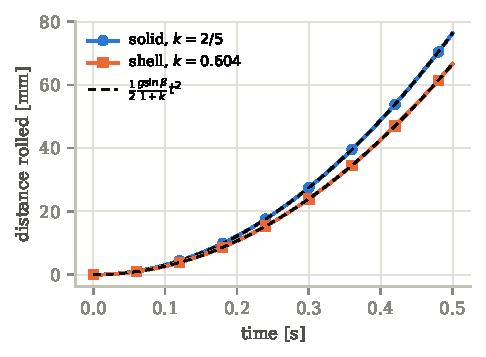
\includegraphics[width=0.48\textwidth]{figures/incline.pdf}\hfill
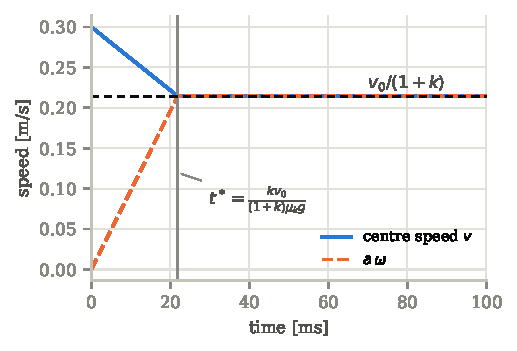
\includegraphics[width=0.48\textwidth]{figures/slide.pdf}\\[4pt]
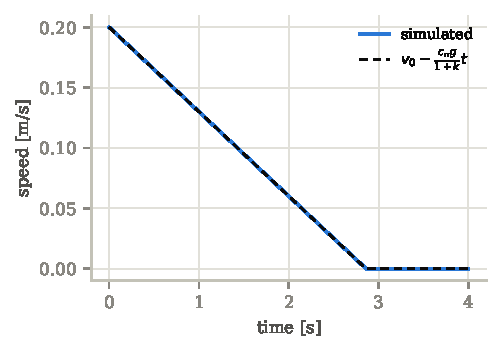
\includegraphics[width=0.48\textwidth]{figures/rolling_resistance.pdf}\hfill
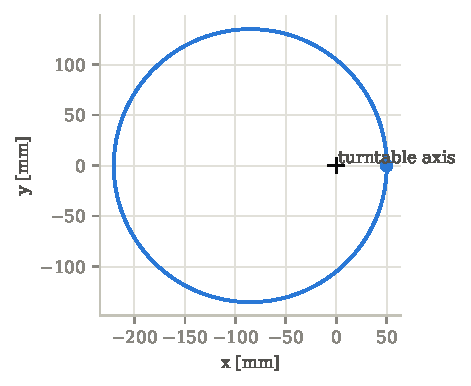
\includegraphics[width=0.36\textwidth]{figures/turntable.pdf}
\caption{Ball dynamics against theory. Top left: distance rolled down a $5^\circ$ incline for a
solid ball and a hollow shell; the shell's larger rolling inertia slows it. Top right: a ball
launched sliding at $0.3\un{m/s}$ starts rolling at $\frac57v_0$. Bottom left: deceleration
under rolling resistance ($c_{rr}=0.01$), then static hold. Bottom right: path of a ball on a
turntable (1 rev/s), one closed orbit every $3.5$ turntable revolutions.}
\label{fig:ball}
\end{figure}

\begin{figure}[h]
\centering
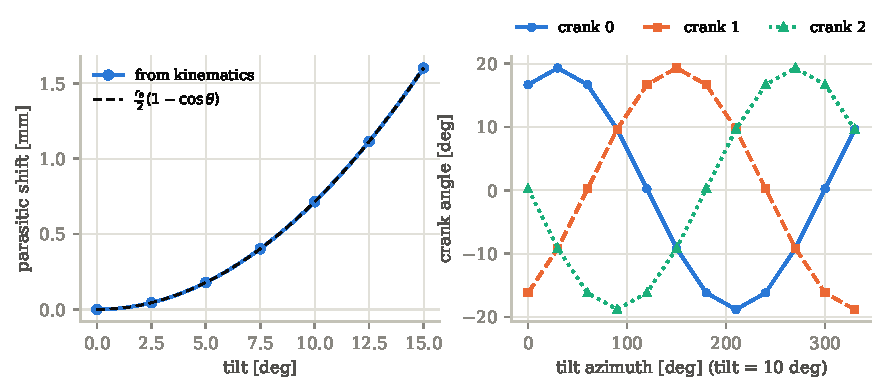
\includegraphics[width=\textwidth]{figures/kinematics.pdf}
\caption{Left: parasitic translation of the joint circle with tilt, against the closed form
\eqref{eq:parasitic}. Right: crank angles for a $10^\circ$ tilt as its azimuth goes round,
the $120^\circ$-shifted pattern of the three legs.}
\label{fig:kin}
\end{figure}

\begin{figure}[h]
\centering
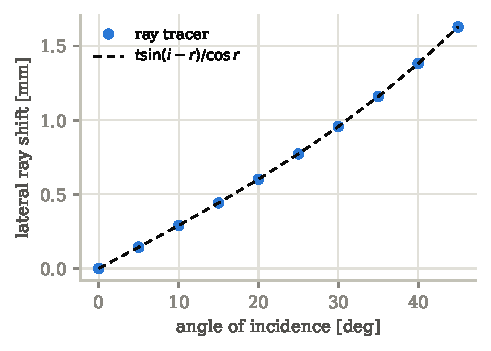
\includegraphics[width=0.48\textwidth]{figures/slab_shift.pdf}\hfill
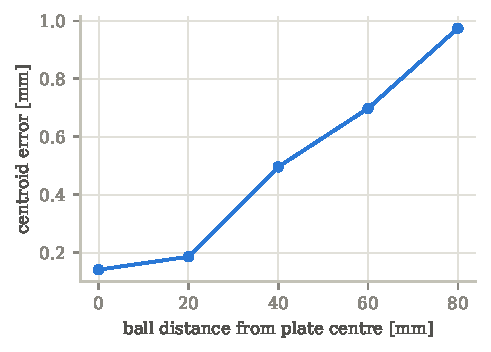
\includegraphics[width=0.48\textwidth]{figures/centroid_bias.pdf}\\[4pt]
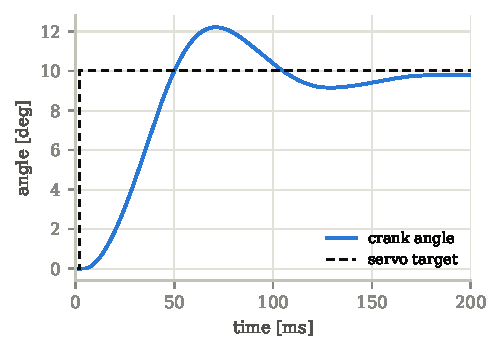
\includegraphics[width=0.48\textwidth]{figures/servo_step.pdf}
\caption{Top left: lateral shift of a camera ray by the plate. Top right: error of the ball
position estimated from the intensity-weighted centroid of its silhouette in a noise-free
render. Perspective and refraction make the silhouette's centroid differ from the projection of
the centre, which is a systematic error a careful tracker has to account for. Bottom: servo step
response ($10^\circ$) under the platform load. The peak speed is $5.3\un{rad/s}$, below the
no-load $7.5\un{rad/s}$, and the crank settles inside the deadband.}
\label{fig:cam}
\end{figure}

%======================================================================
\section{End-to-end demonstration}\label{sec:demo}
%======================================================================
To exercise the whole chain, the closed loop is run through the simulated camera. A simple
dark-blob tracker (threshold, boss masking, intensity-weighted centroid) back-projects the
centroid through the plate. A PD law with a filtered finite-difference velocity estimate
computes the slope angles, and the shared inverse kinematics turns them into servo pulses. This
is the kind of program a student writes. \Cref{fig:closedloop} shows the ball following setpoint
steps; \cref{fig:frames} shows the images the tracker receives. The simulation runs about
$2.7\times$ faster than real time with full image synthesis on a desktop PC.

\begin{figure}[h]
\centering
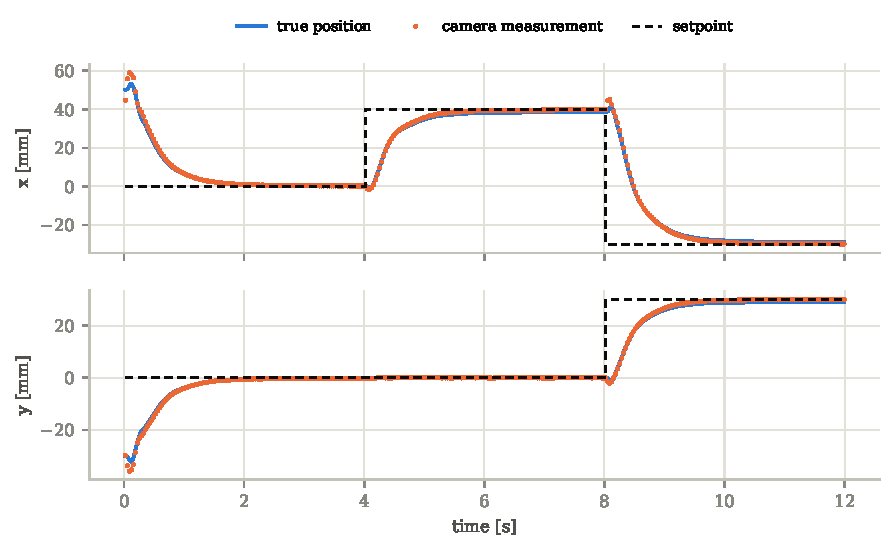
\includegraphics[width=\textwidth]{figures/closed_loop.pdf}
\caption{Closed loop through the simulated camera (30 fps) and servos. The ball starts at
$(50,-30)\un{mm}$ and follows setpoint steps. The final offset of about $1\un{mm}$ comes from
rolling resistance (the dead zone of \cref{sec:ball}) together with the centroid bias.}
\label{fig:closedloop}
\end{figure}

\begin{figure}[h]
\centering
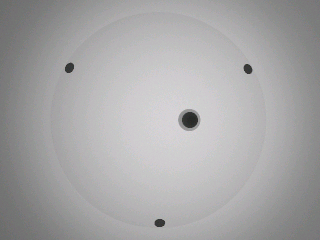
\includegraphics[width=0.48\textwidth]{figures/frame_noisy.png}\hfill
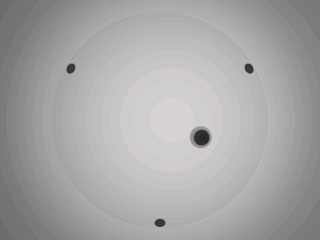
\includegraphics[width=0.48\textwidth]{figures/frame_clean.png}
\caption{Rendered RGB565 frames. Left: during the closed-loop run, with sensor noise. Right: a
noise-free render, where the RGB565 quantisation of the vignetted ceiling shows as rings. The
plate disc is slightly darker than its surroundings because of Fresnel losses, and the three
joint bosses and the steel ball (dark, with a reflective rim) are visible.}
\label{fig:frames}
\end{figure}

%======================================================================
\section{Assumptions and limitations}\label{sec:limitations}
%======================================================================
The following are \emph{not} modelled. Each is a known difference between simulator and
platform.
\begin{itemize}
  \item \textbf{Mechanism}: gear backlash and joint clearances; friction in the passive joints;
        rotational inertia of the rods; flexibility of the plate, rods and base; manufacturing
        tolerances (all legs are identical and ideally placed).
  \item \textbf{Servos}: current limiting and supply-voltage sag under load; temperature
        dependence; the detailed internal control law of a particular servo model.
  \item \textbf{Ball}: departures from sphericity, surface dirt, and variation of friction over
        the plate; the ball's orientation is not tracked (its appearance is rotation-invariant).
  \item \textbf{Camera}: Bayer mosaic and demosaicing, colour response, auto-exposure, lens
        chromatic aberration and flare; multiple scattering in the plate; rods or base entering
        the field of view; the specific sensor---the CAD shows an OV2710 module, whereas the
        ESP32 camera interface supports OV2640/OV5640-class sensors, so the camera parameters are
        generic.
  \item \textbf{Contact}: the ball--plate contact is rigid (no compliance), and impacts are
        instantaneous.
\end{itemize}
Parameters tagged \tagAS{} should be identified on the real platform. Suggested experiments
are: a coast-down on a level plate ($c_{rr}$); the slope at which a resting ball begins to roll
(dead zone, $c_{rr}$); servo step responses with a known load ($\tau_m$, $e_{\mathrm{pb}}$);
camera calibration with a checkerboard \citep{zhang2000flexible} (intrinsics, distortion, pose);
and dark frames and flat fields for the noise model \citep{foi2008practical}.

%======================================================================
\appendix
\section{Parameters}\label{sec:params}
%======================================================================
\begin{table}[h]
\centering
\caption{Physical parameters and their provenance.}
\label{tab:params}
\footnotesize
\setlength{\tabcolsep}{4pt}
\begin{tabular}{llll}
\toprule
Parameter & Value & Source & Note\\
\midrule
Gravity & $9.80665\un{m/s^2}$ & standard & \\
Ball radius / material & $10\un{mm}$ / steel, $7810\un{kg/m^3}$ & \tagCAD{} / \tagAS & $m_b=32.7\un{g}$, $k=2/5$\\
Ball $E$, $\nu$ & $210\un{GPa}$, $0.30$ & typical steel & Hertz contact\\
Plate material & PMMA, $1190\un{kg/m^3}$ & \tagAS & $m_p=188\un{g}$\\
Plate $E$, $\nu$, $n$ & $3.2\un{GPa}$, $0.37$, $1.49$ & typical PMMA & \\
Friction $\mu_s$, $\mu_k$ & $0.45$, $0.40$ & \tagAS & steel on PMMA\\
Rolling resistance $c_{rr}$ & $10^{-3}$ & \tagAS & dead zone $0.057^\circ$\\
Restitution $e$ & $0.5$ & \tagAS & \\
Drag coefficient & $0.47$ & sphere & negligible\\
Crank, rod material & PLA, $1240\un{kg/m^3}$, solid & \tagAS & \\
Servo stall torque, no-load speed & $1.08\un{N\,m}$, $7.48\un{rad/s}$ & \tagDS{} MG996R, 6 V & \\
Servo time constant, friction & $20\un{ms}$, $0.02\un{N\,m}$ & \tagAS & $J_s=2.9\times10^{-3}\un{kg\,m^2}$\\
Servo deadband, prop.\ band, rate & $5\un{\mu s}$, $6^\circ$, $250\un{Hz}$ & \tagDS, \tagAS, \tagAS & \\
PWM & $50\un{Hz}$, $1.22\un{\mu s}$ steps, $500$--$2500\un{\mu s}$ & ESP32-S3 LEDC & \\
Camera & $320\times240$, HFOV $90^\circ$ (pinhole), $30\un{fps}$ & \tagAS & effective $110^\circ$\\
Distortion $k_1,k_2$ & $-0.25$, $0.05$ & \tagAS & \\
Exposure / readout / latency & $6$ / $15$ / $3\un{ms}$ & \tagAS & \\
Full well, read noise & $6000e^-$, $4e^-$ & \tagAS & \\
Time step & $0.25\un{ms}$ & numerical & RK4\\
\bottomrule
\end{tabular}
\end{table}

\bibliographystyle{plainnat}
\bibliography{references}

\end{document}
